\renewcommand{\figurename}{Supplementary Figure}
\setcounter{figure}{0}

\section{Supplementary figures}\label{appendix:suppl-figures}

\begin{figure}[htb!]
     \centering
     \adjustbox{width=0.85\textwidth,center}{%
        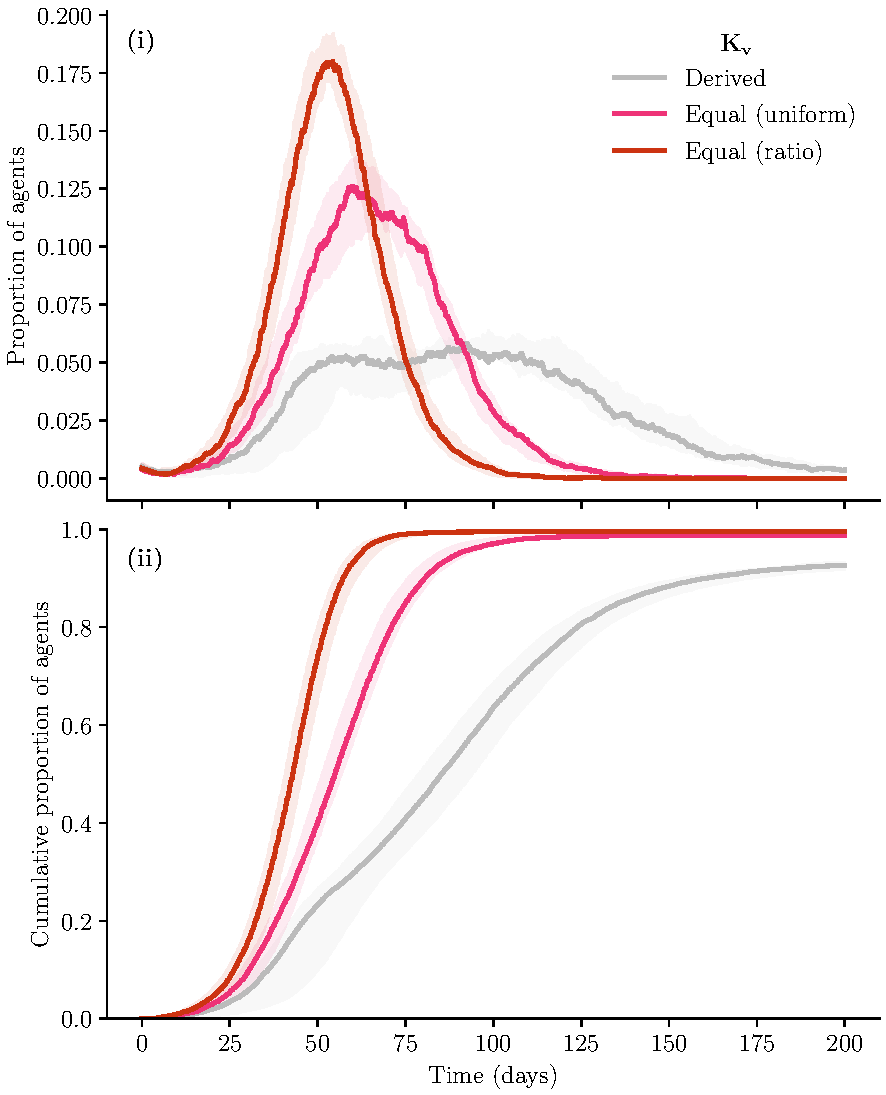
\includegraphics{figures/ch4/k_v_agent_infection.pdf}
    }
    \captionsetup{list=false}
     \bcaption{Proportion of infected agents across varied patch mosquito densities.}{\textbf{(i)} Infection proportions per patch carrying capacity ($K_v$) scenario. \textbf{(ii)} Cumulative infection proportions per patch carrying capacity scenario. Homogeneous mosquito distributions across patches in the extended model led to distinct initial epidemic waves not seen in the derived case.}
    \label{fig:ch4-k-v-infs}
\end{figure}

\begin{figure}[htb!]
     \centering
     \adjustbox{width=0.85\textwidth,center}{%
        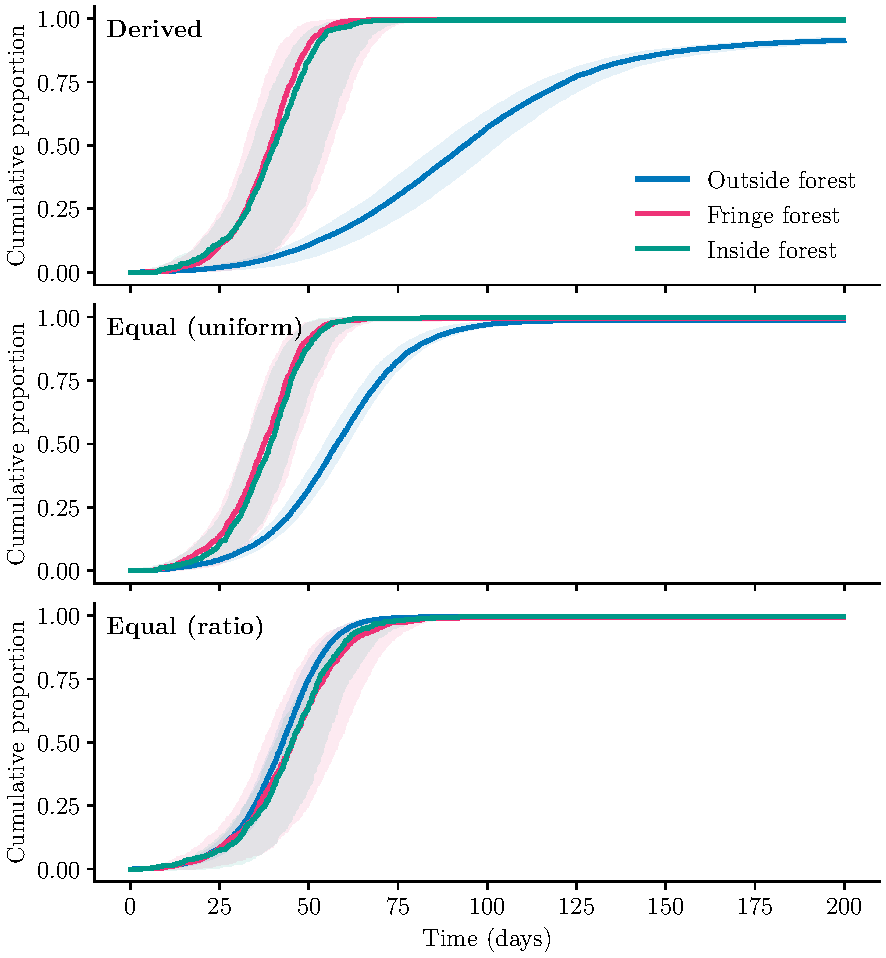
\includegraphics{figures/ch4/k_v_cum_infected_agents.pdf}
    }
    \captionsetup{list=false}
     \bcaption{Cumulative proportions of agents infected across varied patch mosquito densities.}{As patches became more equal in terms of mosquito density, infections in the outside forest patch approximated that of the fringe and inside forest patches.}
    \label{fig:ch4-k-v-patch-infs}
\end{figure}

\begin{figure}[h]
     \centering
     \adjustbox{width=1.1\textwidth,center}{%
        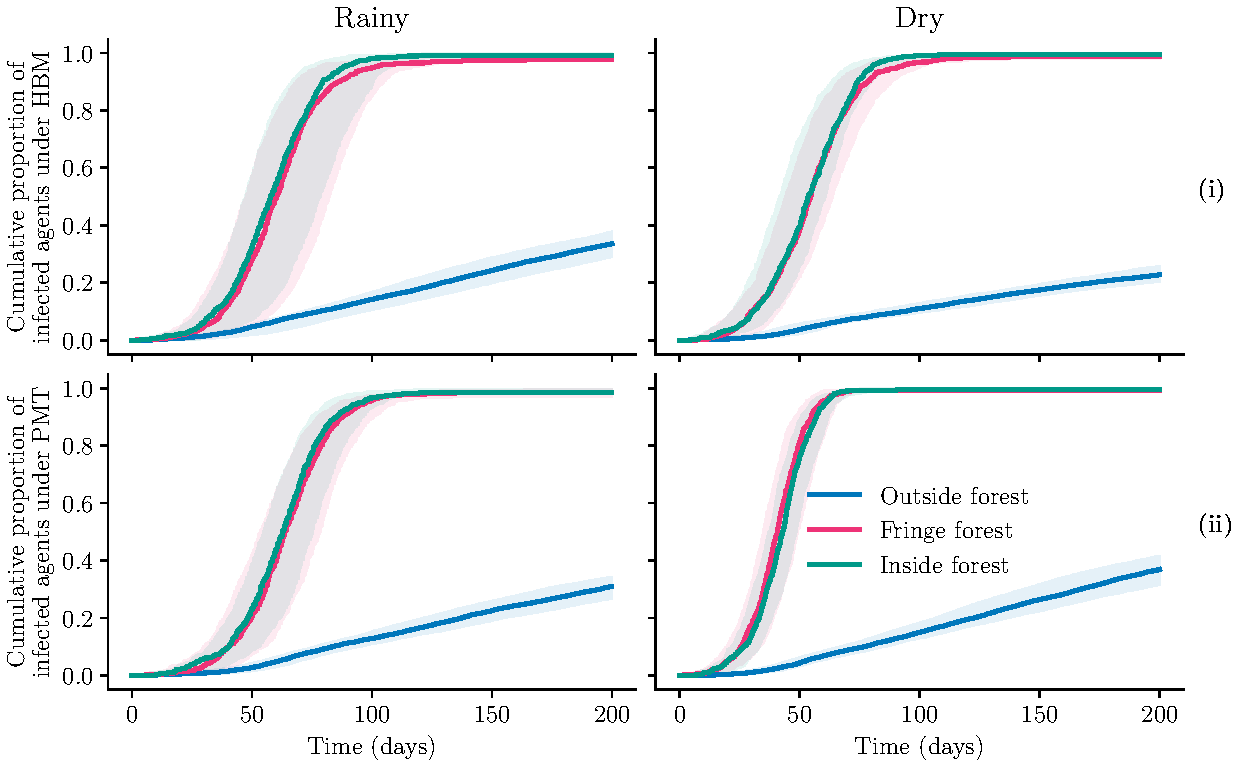
\includegraphics{figures/ch5/2-cum-patch.pdf}
    }
    \captionsetup{list=false}
     \bcaption{Cumulative infections across patches for BCTs and simulated seasons.}{\textbf{(i)} Cumulative infections under the Health Belief Model (HBM) implementation. \textbf{(ii)} Cumulative infections under the Protection Motivation Theory (PMT) implementation. Rainy season infections under both behaviour change theories (BCTs) are similar, while the dry scenario under the PMT reaches higher infection levels faster than under the HBM.}
    \label{fig:ch5-cum-patch}
\end{figure}

\begin{figure}[h]
     \centering
     \adjustbox{width=1.1\textwidth,center}{%
        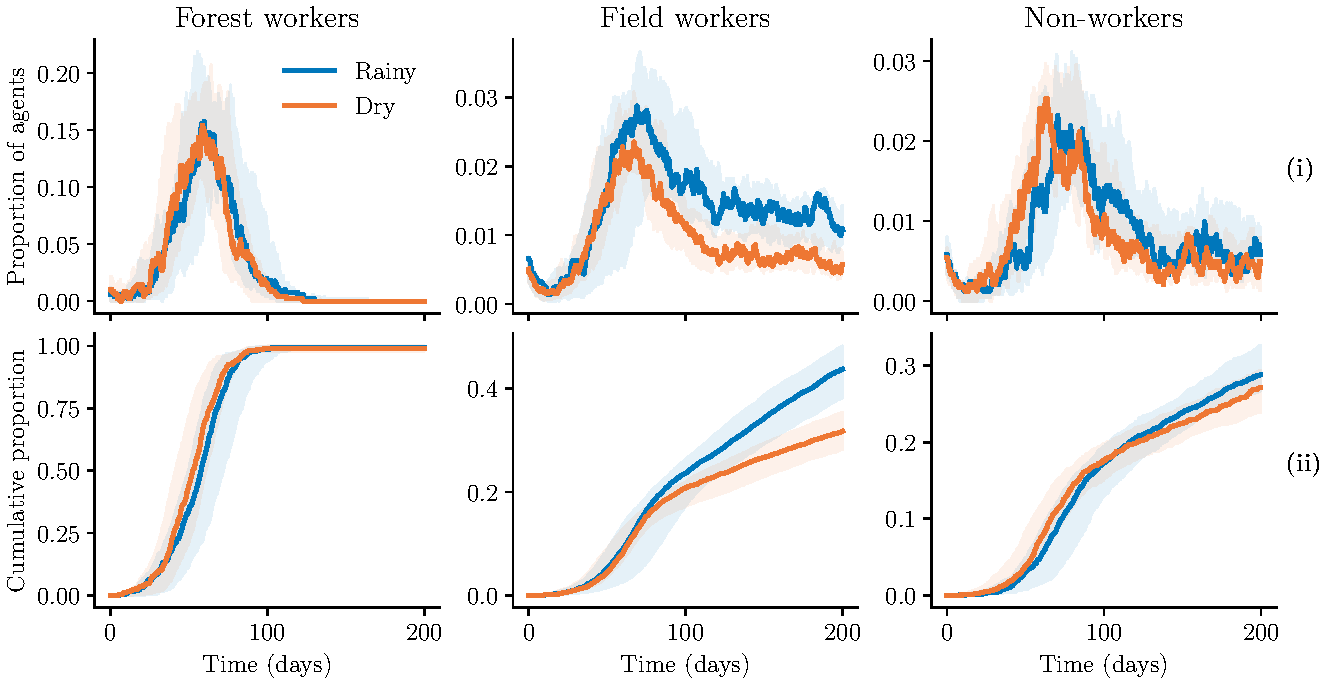
\includegraphics{figures/ch5/7-hbm-risk-groups.pdf}
    }
    \captionsetup{list=false}
     \bcaption{Seasonal infection dynamics across occupational risk groups under the HBM implementation.}{\textbf{(i)} Historical infection counts over time. \textbf{(ii)} Cumulative infection proportions over time. Infection dynamics are similar for forest workers and non-workers across seasons, but field workers have reduced exposure to disease in the dry season. Note that $y$-axes are not shared between plots.}
    \label{fig:ch5-hbm-risk-groups}
\end{figure}

\begin{figure}[h]
     \centering
     \adjustbox{width=1.1\textwidth,center}{%
        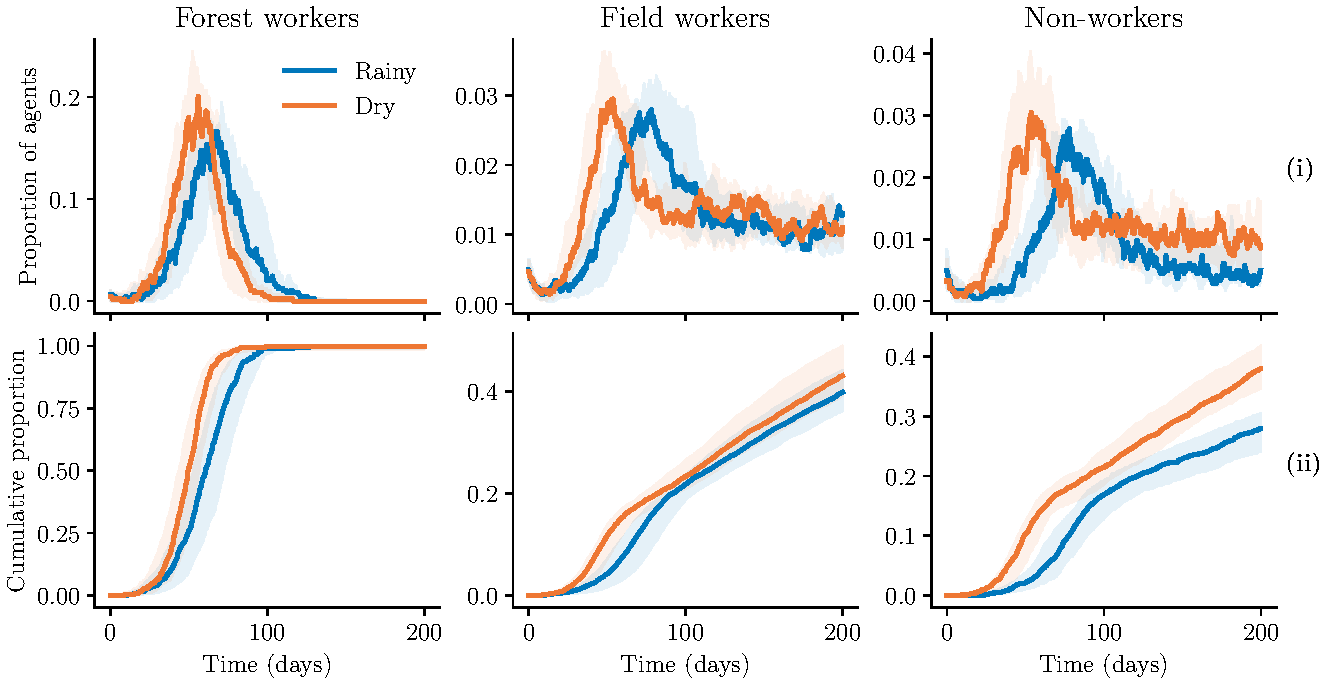
\includegraphics{figures/ch5/8-pmt-risk-groups.pdf}
    }
    \captionsetup{list=false}
     \bcaption{Seasonal infection dynamics across occupational risk groups under the PMT implementation.}{\textbf{(i)} Historical infection counts over time. \textbf{(ii)} Cumulative infection proportions over time. Across all occupational risk groups, the dry season leads to more severe infection dynamics compared to the rainy season, unlike the HBM. Note that $y$-axes are not shared between plots.}
    \label{fig:ch5-pmt-risk-groups}
\end{figure}

\begin{figure}[h]
     \centering
     \adjustbox{width=1.2\textwidth,center}{%
        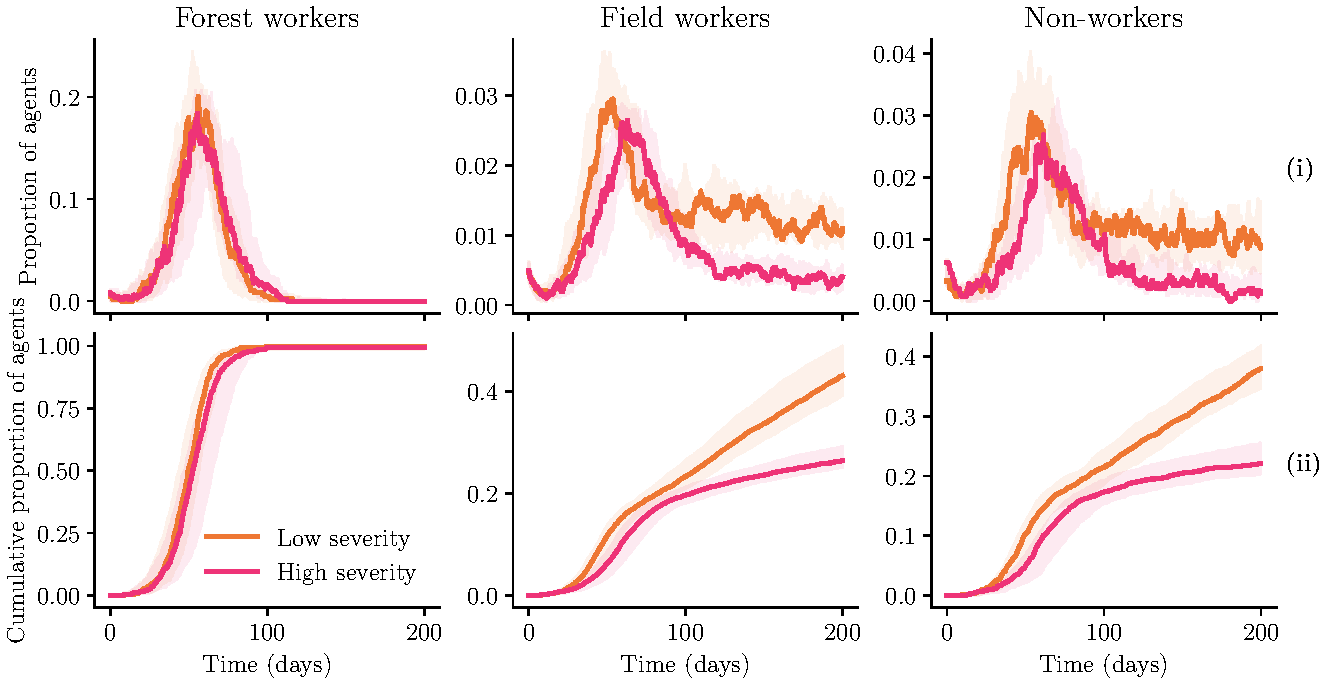
\includegraphics{figures/ch5/ex2-occupations.pdf}
    }
    \captionsetup{list=false}
     \bcaption{Infection dynamics across low and high perceived severity during the dry season under PMT.}{\textbf{(i)} Historical infection counts over time. \textbf{(ii)} Cumulative infection proportions over time. When perceived severity is low in the dry season, infection dynamics are more severe compared to high perceived severity, although this effect is weaker for forest workers. Note that $y$-axes are not shared between plots.}
    \label{fig:ex2-occupations}
\end{figure}




